\documentclass{beamer}
\hypersetup{
	colorlinks=true,
	linkcolor=blue,
	filecolor=magenta,      
	urlcolor=cyan,
	pdftitle={Overleaf Example},
	pdfpagemode=FullScreen,
}

\usepackage{caption}
\captionsetup{labelformat=empty, textfont=it}

% Chargement du logo
\logo{\includegraphics[height=0.75cm]{images/logo_enseirb.jpg}}

% Choix du thème
\usetheme{CambridgeUS}  % Thème de présentation
\usecolortheme{dolphin} % Thème de couleurs

% Informations sur la présentation
\title{Séance du 24/01}
\author{Projet S8: TRACK}
\institute[T2, Enseirb-Matmeca]{Département Télécommunication\\Enseirb-Matmeca, Bordeaux}
\date{\today}

% Début du document
\begin{document}
	
	% Page de titre
	\begin{frame}
		\titlepage
	\end{frame}
	
	% Introduction
	\begin{frame}
		\frametitle{Ordre du Jour}
		\begin{itemize}
			\item Présentation des avancées Traitement du signal
			\item Présentation des résultats d'approches IA
			\item Questions 
		\end{itemize}
	\end{frame}
	
	% Compte rendu des avancées
	\begin{frame}
		\frametitle{Compte rendu des avancées}
		\begin{itemize}
			\item MRU :
			\begin{itemize}
				\item[\hspace{1cm}] Résultats expérimentaux et déductions 
				\item[\hspace{1cm}] \[R_{xx}(0) = \frac{2\sigma^2}{T_{ech}^3} \]
				\item[\hspace{1cm}] Blocage calcul (Stationarité au Sens Large | Autocorrélation) 
			\end{itemize}
			\item MUA :
			\begin{itemize}
				\item[\hspace{1cm}] Résultats expérimentaux et déductions 
				\item[\hspace{1cm}] \[R_{xx}(0) = \frac{2\sigma^4}{3T_{ech}}\]
				\item[\hspace{1cm}] Blocage calcul (Stationarité au Sens Large | Autocorrélation) 
			\end{itemize}
			\item Approches IA
			\begin{itemize}
				\item[\hspace{1cm}] Résultats réseaux réccurents (LSTM)
			\end{itemize}
		\end{itemize}
	\end{frame}
	
	\begin{frame}{Résultats LSTM}
        \begin{columns}
            \column{0.5\textwidth}
            \centering
            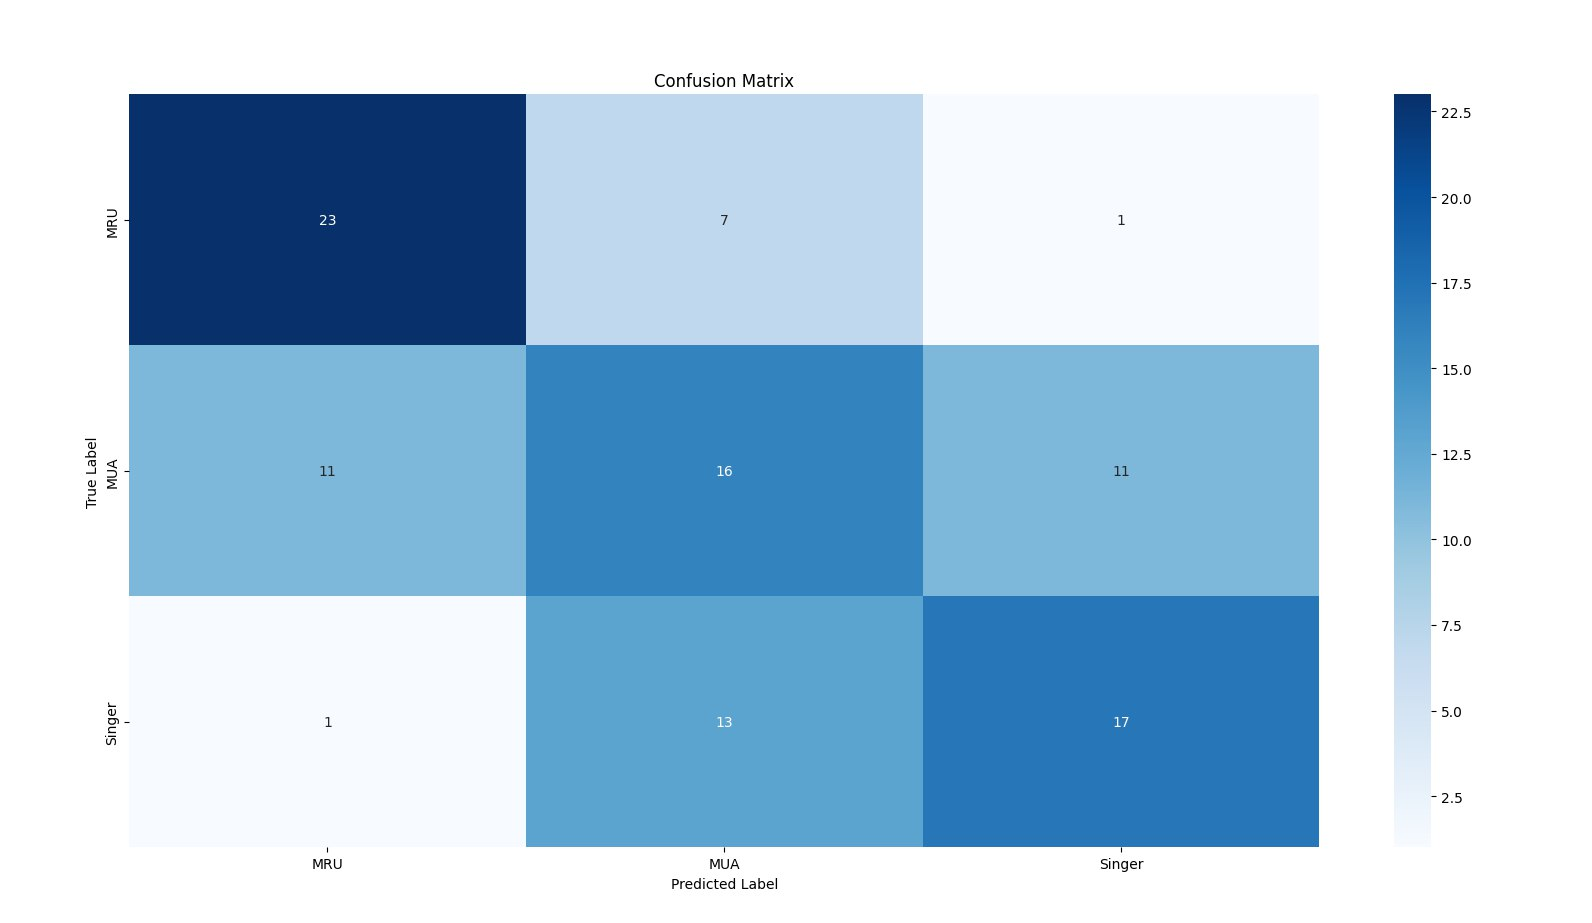
\includegraphics[width=0.9\linewidth]{Images/lstm_test.jpeg}
            \begin{itemize}
                \item Nombre de trajectoires : $190 000$
                \item Longueur trajectoire : $15 - 3600$
                \item $T_{ech}=1$ ; $\sigma^2 \in [0,001; 0,1]$
                \item $\alpha = 0,1$
            \end{itemize}
    
            \column{0.5\textwidth}
            \centering
            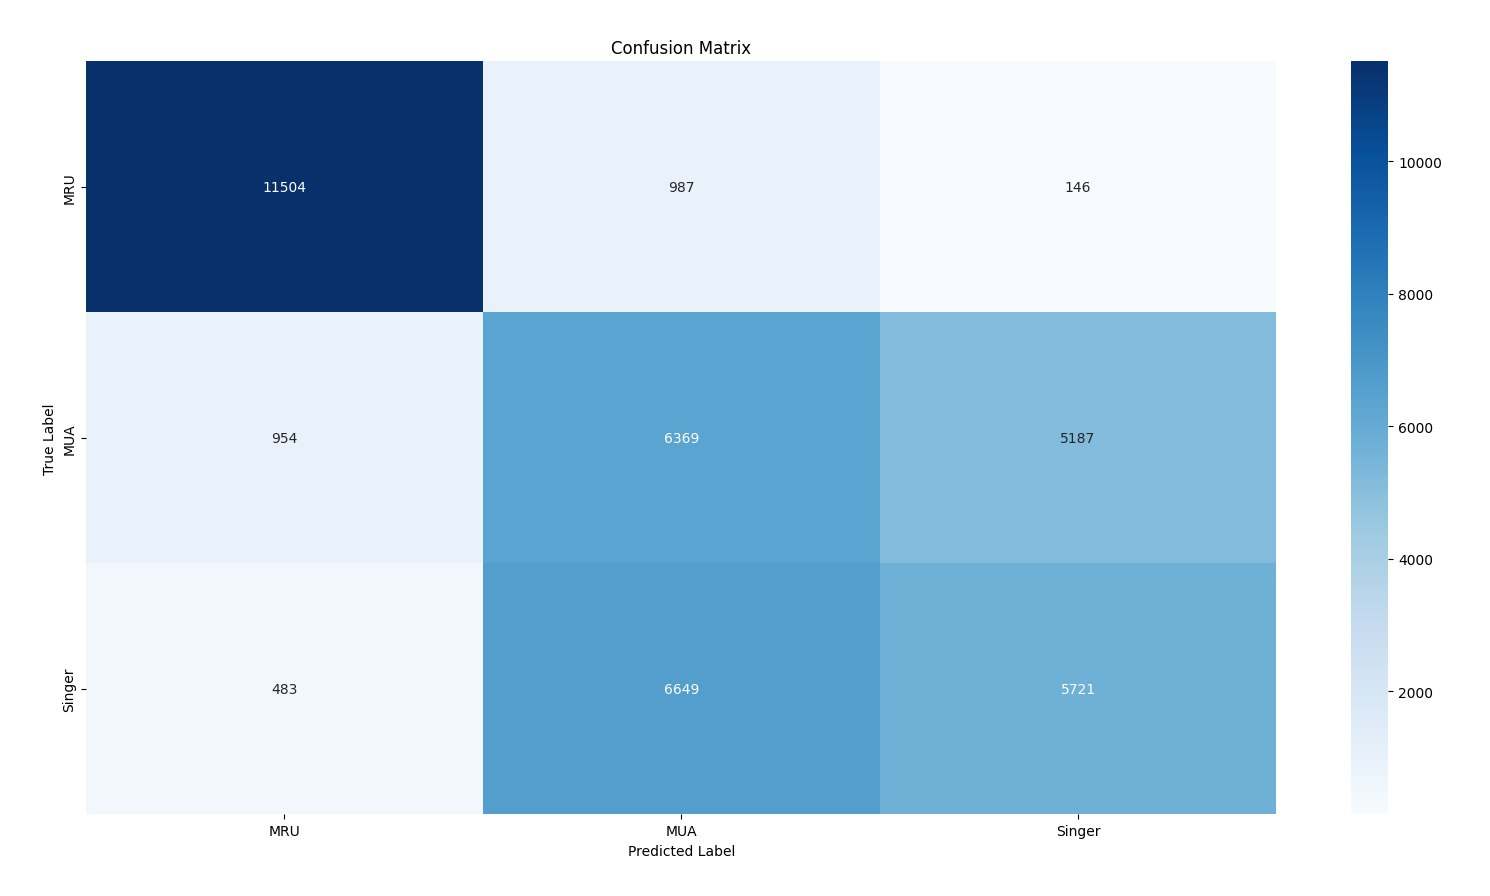
\includegraphics[width=0.9\linewidth]{Images/lstm_long.jpeg}
            \begin{itemize}
                \item Nombre de trajectoires : $500$
                \item Longueur trajectoire : $50-150$
                \item $T_{ech}=0,1$ ; $\sigma^2 \in [1e-3; 0,05]$
                \item $\tau \in [1; 300]$ ; $\sigma_m^2 \in [1e-4; 1]$
            \end{itemize}
        \end{columns}
    \end{frame}

    \begin{frame}{Questions}
        \Huge Questions
    \end{frame}
	
	% Fin de la présentation
\end{document}
